\documentclass[14pt]{extarticle}
\usepackage[
left=25mm,
top=20mm,
right=15mm,
bottom=20mm,
]{geometry}

%\usepackage{graphicx}
\usepackage[pdftex]{graphicx}
\usepackage[utf8x]{inputenc}
\usepackage[russian]{babel}
\usepackage[T1]{fontenc}
\usepackage{float}
\usepackage{listings}
\usepackage{cite}
\usepackage{hyperref}
\usepackage{etoolbox}
\usepackage{amsmath}
\usepackage[linesnumbered,boxed]{algorithm2e}
\sloppy

\lstdefinelanguage{llang}{
keywords={skip, do, while, read, write, if, then, else},
sensitive=true,
basicstyle=\small,
commentstyle=\scriptsize\rmfamily,
keywordstyle=\ttfamily\underbar,
identifierstyle=\ttfamily,
basewidth={0.5em,0.5em},
columns=fixed,
fontadjust=true,
literate={->}{{$\to$}}1
}

\lstset{
language=llang
}
\makeatletter
%\renewcommand{\@biblabel}[1]{#1.} % Заменяем библиографию с квадратных скобок на точку:
\makeatother
\gappto\captionsrussian{\renewcommand{\contentsname}{Оглавление}}
\renewcommand\baselinestretch{1.5}
\renewcommand{\lstlistingname}{Листинг}

\begin{document}

\begin{titlepage}
\thispagestyle{empty}
\def\baselinestretch{1.0}
\begin{center}
	{САНКТ-ПЕТЕРБУРГСКИЙ ГОСУДАРСТВЕННЫЙ УНИВЕРСИТЕТ \\ \vskip 0.3em {\large Математико-механический факультет \\ \vskip 0.7em{\large Кафедра системного программирования \\}}}
    \vspace*{0.15\textheight}
    {\large Гудиев Артур Владимирович}
    
    \vskip 2em
    {\huge Реализация графической части интерпретатора языка PostScript}
    
    \vskip 1em
    {\large Курсовая работа} \\
    \vskip 2em
    {\normalsize \raggedleft 
    Зав. кафедрой:\\
    д.ф.-м.н., проф. А.Н. Терехов
    \\[3em]
    Научный руководитель:\\
    к.ф.-м.н. Д.Ю. Булычев
    \\[3em]
    %Рецензент:\\
    %Неизвестно \\
    \vspace*{0.08\textheight}
    {\centering Санкт-Петербург \\ 2014}
    }
\end{center}
\end{titlepage}

\tableofcontents
\thispagestyle{empty} 
\pagebreak

\iffalse
\documentclass[a4paper, 12pt]{article}
\usepackage[
left=25mm,
top=20mm,
right=25mm,
bottom=20mm,
]{geometry}
\usepackage{mathtext}
\usepackage{url}
\usepackage{cmap}
\usepackage[utf8x]{inputenc}
\usepackage[russian]{babel}
\usepackage[T2A]{fontenc}
\usepackage{amsmath,amssymb,amsthm,amscd,amsfonts}

\usepackage{bbm}
\usepackage[boxed]{algorithm2e}

\usepackage{color} %% это для отображения цвета в коде
\usepackage{listings} %% собственно, это и есть пакет listings

\usepackage{caption}
\usepackage[pdftex]{graphicx}
\DeclareCaptionFont{white}{\color{black}} %% это сделает текст заголовка белым
%% код ниже нарисует серую рамочку вокруг заголовка кода.
\DeclareCaptionFormat{listing}{\colorbox{white}{\parbox{\textwidth}{#1#2#3}}}
\captionsetup[lstlisting]{format=listing,labelfont=white,textfont=white}

\SetAlgorithmName{Алгоритм}{алгоритм}{Список алгоритмов}
\SetKwInput{KwResult}{Результат}
\SetKwInput{KwData}{Входные данные}
\fi

\section*{Введение}
\addcontentsline{toc}{section}{Введение}
\sloppy
  
 
Язык PostScript – интерпретируемый графический язык программирования, который создавался с целью представления цифровой графики в машинонезависимой форме\cite{plrm}. PostScript предоставляет возможности вывода векторной и растровой графики, а также печати текста. Интерпретатор PostScript считывает программу и выводит результат на экран или принтер. 
  
Интерпретатор PostScript оперирует сущностями, которые называются объектами PostScript. У каждого объекта есть такие свойства, как тип, значение и атрибуты. У интерпретатора PostScript есть своя среда исполнения, которая состоит из стеков, виртуальной памяти и графической среды исполнения. Виртуальная память представляет собой хранилище для значений объектов PostScript, а сами объекты находятся в стеках. Графическая среда выполнения описывает графическое состояние исполняемой программы.

Графическое состояние содержит  такие параметры, как ширину линии,  цвет,  текущий путь, текущую матрицу преобразования и  ограничивающий путь.  Применяя операторы рисования и построения пути, можно нарисовать линии, дуги и кривые Безье \cite{graphics}, залить заданным цветом внутреннюю область  пути, ограничить область рисования, преобразовать текущую систему координат.


В языке PostScript есть графические операторы, которые действуют на графическое состояние. Такие операторы могут, например, поменять масштаб рисования, задать цвет или ширину линии. Кроме того есть операторы, сохраняющие текущее графическое состояние, в котором хранятся основные графические параметры. По сохраненному состоянию можно задать текущее графическое состояние таким, каким оно было в момент сохранения.  

На сегодняшний день существует большое количество платформ, у каждой из которых есть свои отличительные особенности. Реализация интерпретатора PostScript для каждой платфромы довольно затруднительна, поэтому  необходимо обеспечить переносимость интерпретатора. 

 Java – объектно-ориентированный язык программирования. Программы на Java переводятся компилятором Java (javac)  в специальный байт-код Java. Виртуальная машина Java (сокращенно Java VM, JVM) – основная часть исполняющей системы Java, так называемой Java Runtime Environment (JRE). Виртуальная машина Java интерпретирует байт-код. В настоящий момент виртуальная машина Java широко распространена. Следовательно, программа, написанная на языке Java, может быть исполнена на большом количестве платформ вне зависимости от архитектуры компьютера. Язык Java предоставляет основные графические возможности для рисования. 
 
Целью курсовой работы является реализация графической части интерпретатора языка PostScript.  Необходимо реализовать на языке Java графическую среду исполнения для интерпретатора программ PostScript. Интерпретатор должен поддерживать основные графические операторы, отображать графическое состояние на экране согласно спецификации.


\pagebreak

\section{Общие сведения о языке PostScript}
Язык PostScript – это динамический интерпретируемый язык программирования, который содержит стандартное множество типов данных (числа, массивы и строки), основные элементы управления (условия, метки и процедуры), а также некоторые необычные особенности, например, словари. 


Язык PostScript имеет следующие графические возможности, содержащиеся в среде языка:
\begin{itemize}
\item изображения произвольных графических объектов, построенных из отрезков, дуг и кубических кривых;
\item графические операторы, позволяющие обрисовывать формы линиями произвольной ширины, залить область любым цветом или использовать ее в качестве ограничивающего пути;
\item координатную систему, которая поддерживает все комбинации линейных преобразований.
\end{itemize}

 
Интерпретатор  языка PostScript действует, исполняя последовательность объектов. Объекты, которые нужно исполнить, могут придти из двух источников:
\begin{itemize}
\item Поток символов может анализироваться согласно синтаксическим правилам языка, при этом символы группируются в токены, а затем из одного или более токенов создаются объекты. Как только объект проанализирован, он немедленно исполняется. 
\item Объекты, ранее сохраненные в массиве, могут быть исполнены последовательно. Такой массив называется \textit{процедурой}.
\end{itemize} 
 
\subsection{Модель данных}
Все данные, доступные программе PostScript, существуют в форме объектов. У каждого объекта есть \textit{тип} и \textit{значение}. %и \textit{атрибуты}. 

Объекты бывают \textit{простые} и \textit{сложные}. Простой объект является константой, его тип, значение и атрибуты неизменно соединены вместе и не могут быть изменены. У сложных объектов значения хранятся отдельно от самих объектов. 

Важное отличие между \textit{простыми} и \textit{сложными} объектами проявляется при операциях копирования объектов. При копировании \textit{простого} объекта все его части копируются вместе. При копировании \textit{сложного} объекта \textit{значение} не копируется, вместо этого исходный и скопированный объекты разделяют одно значение.
Следовательно, если значение некоторого исходного объекта изменилось, то оно изменилось у всех объектов, разделяющих одно значение вместе с исходным.

%У каждого объекта есть один или несколько атрибутов, которые влияют на поведение объекта при его исполнении. Каждый объект может быть \textit{литеральным %(literal)}, при этом интерпретатор рассматривает его только как данные и кладет его на стек операндов,  или \textit{исполняемым (executable)}, так что %интерпретатор исполняет такой объект.

%Другим атрибутом является тип доступа к объекту. Есть четыре типа доступа к объекту: неограниченный \textit{Unlimited}, для чтения и исполнения  \textit{Read-only}, только для исполнения \textit{Execute-only} и тип доступа \textit{None}, при котором запрещаются все операции.

\subsubsection*{Типы данных и объекты}

Объекты в PostScript бывают простые и сложные. Ниже приведены виды простых и сложных объектов в PostScript:

\begin{center}

\begin{tabular}[t]{|p{12em}|p{12em}|}
\hline
Простые объекты & Сложные объекты\\
\hline
boolean & array\\
integer & dictionary\\
mark & gstate\\
name & save\\
null & string\\
operator & \\
real & \\
\hline
\end{tabular}

\end{center}
$$ $$

\textit{Числа} в языке PostScript бывают:
\begin{itemize}
\item знаковые целые (\textit{integer}), такие как \texttt{123, -76, 0, +17};
\item вещественные (\textit{real}), такие как \texttt{-.002, 56.7, 123.6e10}.
\end{itemize} 

Для логических выражений поддерживаются \textit{логические} объекты со значениями \texttt{true} и \texttt{false}. 

Объекты \textit{операторы} (\textit{operator})  представляют некоторые встроенные в язык действия. \textit{Операторы} связаны со своими именами (например, \texttt{fill, gsave и rlineto}) в стандартном словаре \texttt{systemdict}.

%\textit{Строка} в PostScript (\textit{string}) --- это буквенный текст, заключенный между "(" и ")".

Любой токен, состоящий из стандартных символов, который нельзя рассматривать как число (например, \texttt{"abc"$,$ "Offset"$,$ "23A"}) является \textit{именем} или \textit{именным объектом} (\textit{name}). 
Символ /, являющийся префиксом некоторого имени, представляет \textit{буквенное имя} (\textit{literal name}), например "\texttt{/variable}".

\textit{Массивом} (\textit{array}) является последовательность объектов PostScript, заключенная между "[" и "]" $ $, например "\texttt{ [ 123  /abc (xyz) ]}".

Похожий синтаксис есть у \textit{процедур } (\textit{procedure}), которая является \textit{исполняемым массивом}. \textit{Процедура} --- это последовательность объектов, заключенная между "\{" и "\}"$ $ , например, "\texttt{\{ add 2 div \}}".

Последовательность пар, состоящих из ключа и значения, которая заключена между "$ $<<" и "$ $>>"$ $ , определяет словарь в PostScript, например, "\texttt {<< (number) 17 (string) (world) (array) [1 2]  >>}"

%Кроме того, есть объекты \textit{метки} (\textit{mark}), которые позволяют сконструировать сложные объекты, например, \texttt{ "$ $<<"$ $, "\}"$ $, "("$ $, "]" }. 
Для сохранения состояния памяти интерпретатора существуют объекты \textit{сохранения} (\textit{save}), которые создаются оператором \texttt{save} и с помощью которых можно восстановить состояние памяти оператором \texttt{restore}. Также есть объект \textit{графического состояния} (\textit{gstate}), предназначенный для использования графических возможностей языка PostScript.

\subsection{Структура памяти интерпретатора}
Данные в языке PostScript представлены в виде объектов. Важное место в языке занимают стеки и виртуальная память, поскольку все объекты хранятся на стеках, а виртуальная память предоставляет место для хранения значений сложных объектов.
\subsubsection{Стеки }
Интерпретатор PostScript управляет стеками, которые представляют исполняемое состояние программы. 
\begin{itemize}
\item Стек операндов содержит произвольные объекты PostScript, являющиеся операндами или результатами некоторых исполняемых операторов.
\item Стек словарей содержит только словари. В нем содержатся три стандартных словаря \texttt{systemdict}, \texttt{userdict} и \texttt{globaldict}.
\item Стек исполнения содержит исполняемые объекты, находящиеся в промежуточной стадии исполнения.
\item Графический стек хранит только объекты графического состояния.
\end{itemize}

\subsubsection{Управление памятью}
В языке PostScript предусмотрено хранилище для значений \textit{сложных} объектов --- \textit{виртуальная память}. \textit{Сложный} объект имеет ссылку на свое \textit{значение}. \textit{Виртуальная память} подразделяется на \textit{локальную} и \textit{глобальную}.
Основным отличием является то, что операторы сохранения \texttt{save} и восстановления \texttt{restore} состояния памяти влияют только на \textit{локальную виртуальную память}. 
Для освобождения памяти, выделенной для объектов, которые уже не используются, используется сборщик мусора. 

\subsection{Графика}
Воздействовать на графическую состояние программы можно с помощью графических операторов. В языке PostScript графические операторы можно разделить на три группы: операторы построения пути, рисующие операторы и операторы координатной системы и матрицы преобразования.

Интерпретатор PostScript неявно поддерживает \textit{текущую страницу}, которая накапливает результаты работы рисующих операторов. В начале исполнения программы \textit{текущая страница} пуста. Как только некоторый рисующий оператор исполняется, он кладет соответствующие метки на \textit{текущую страницу}. При перекрытии каждое новое изображение загораживает все старые. Как только \textit{текущая страница} сформирована, вызов оператора \textit{showpage} изображает все накопленные результаты графических операторов на экране и очищает \textit{текущую страницу}.

Общий алгоритм рисования для программ PostScript можно описать следующим образом:

\begin{itemize}
\item [1. ] формирование пути с помощью операторов построения пути;
\item [2. ] задание некоторых неявных параметров при необходимости;
\item [3. ] вызов рисующих операторов.
\end{itemize} 



Интерпретатор PostScript поддерживает внутреннюю структуру данных --- \textit{графическое состояние}, хранящую графические параметры управления, такие как текущую позицию \texttt{position}, текущую матрицу преобразования \texttt{cTM}, текущий путь \texttt{path}, ограничивающий путь \texttt{clipping path}, цвет \texttt{color}, ширину линии \texttt{line width}, форму конца линии \texttt{line cap}, форму соединения отрезков \texttt{line join} и параметр пунктирности линии \texttt{dash pattern}.


Язык PostScript определяет декартову систему координат, которую программы могут использовать, чтобы определить расположение произвольной точки на странице.  
\textit{Текущая позиция} представляет собой пару вещественных координат. Многие графические операторы (например, \texttt{lineto, moveto, rcurveto}) неявно используют \textit{текущую позицию} для рисования.

Систему координат можно изменять с помощью линейных преобразований. Линейные преобразования системы координат PostScript представлены в виде \textit{текущей матрицы преобразования} \texttt{cTM}, представленной в виде массива из шести чисел [ $a, b, c, d, t_x, t_y$ ]:
\[
\begin{bmatrix}
a & b & 0 \\ c & d & 0 \\ t_x & t_y & 1
\end{bmatrix}
\]
Такая матрица определяет относительные координаты, которые выражаются через абсолютные:
$$ x' = ax + cy + t_x $$
$$   y' = bx + dy + t_y $$ 
В языке PostScript определены такие линейные преобразования, как перенос, поворот и масштаб. Каждое преобразование определяется соответствующей матрицей. 

Матрица сдвига на вектор $(t_x, t_y)$:
\[
\begin{bmatrix}
1 & 0 & 0 \\ 0 & 1 & 0 \\ t_x & t_y & 1
\end{bmatrix}
\]

Матрица изменения масштаба, в которой параметры $s_x$ и $s_y$ определяют масштаб по осям $x$ и $y$ соответственно:
\[
\begin{bmatrix}
s_x & 0 & 0 \\ 0 & s_y & 0 \\ 0 & 0 & 1
\end{bmatrix}
\]

Матрица поворота на угол $\theta$:
\[
\begin{bmatrix}
\cos \theta & \sin \theta & 0 \\ -\sin \theta & \cos \theta & 0 \\ 0 & 0 & 1
\end{bmatrix}
\]

 Операторы переноса \texttt{translate}, поворота \texttt{rotate} и масштаба \texttt{scale} изменяют \textit{текущую матрицу преобразования}, так что новая матрица является произведением матрицы соответствующего преобразования и исходной матрицы: 
\[ \texttt{новая матрица} = \texttt{преобразование} \times \texttt{исходная матрица} \]
Оператор \texttt{transform}, принимающий один параметр --- массив из шести чисел,--- переопределяет новую \textit{матрицу преобразования}. 

В языке PostScript есть объекты \textit{пути}, характеризующие графические объекты. Программы используют \textit{пути} для рисования линий, определения форм закрашиваемой области и границ для ограничения области рисования. 
Объект \textit{пути} состоит из связанных подпутей, построенных из прямых линий, кубических кривых и дуг эллипсов. Изначально есть только один подпуть, к которому могут добавляться новые элементы, не нарушающие его связанность. При попытке добавления элемента, нарушающего связанность, создается новый подпуть, и все новые элементы добавляются уже к нему, таким образом все подпути объекта \textit{пути} остаются связанными. В графическом состоянии языка PostScript есть два объекта пути: \textit{текущий путь} и \textit{ограничивающий путь}. 

\textit{Текущиий путь} можно изменить, используя операторы перемещения текущей позиции ( \texttt{moveto} и \texttt{rmoveto}), присоединения к пути отрезка (\texttt{lineto} и \texttt{rlineto}), различных дуг (\texttt{arc} и \texttt{rarc}), кубических кривых Безье (\texttt{curveto} и \texttt{rcurveto}), а также оператор замыкания текущего связанного подпути \texttt{closepath}.

Ограничивающий путь используется с помощью оператора пересечения текущего пути и текущего ограничивающего пути \texttt{clip} и оператора замены текущего пути копией текущего ограничивающего пути \texttt{clippath}.

Ширина линии представляет собой число и может быть изменена с помощью оператора \texttt{setlinewidth}.

Форма конца линии также представлена числом, принимающим три значения: 0, 1 и 2. Присвоить значение можно с помощью оператора \texttt{setlinecap}. Каждому числу соответствует своя форма конца:
\begin{itemize}
\item [0 ---] стыковой конец;
\item [1 ---] круглый конец;
\item [2 ---] выдвинутый прямоугольный конец.
\end{itemize} 

\begin{figure} [h]
\center{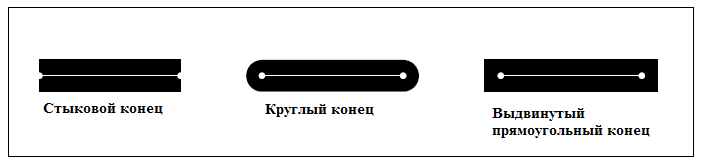
\includegraphics[width=360pt]{linecap.png}}
\caption{Формы параметров конца линии}\label{pic_linecap}
\end{figure}

Форма соединения отрезков в PostScript характеризуется числом, принимающим три значения: 0, 1 и 2. Присвоить значение можно с помощью оператора \texttt{setlinejoin}. Для каждого ччисла определена своя форма соединения:
\begin{itemize}
\item [0 ---] соединение под углом $45^{\circ} $;
\item [1 ---] круглое соединение;
\item [2 ---] скошенное соединение.
\end{itemize} 

\begin{figure} [h]
\center{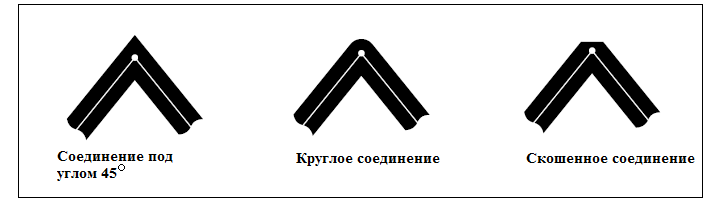
\includegraphics[width=360pt]{linejoin.png}}
\caption{Формы параметров соединения отрезков}\label{pic_linejoin}
\end{figure}

Параметр пунктирности задается с помощью двух элментов: массива, в котором числа поочередно показывают, сколько пикселей нужно заштриховать, а сколько пропустить, и начального сдвига, задаваемого целым числом.

\begin{figure} [h]
\center{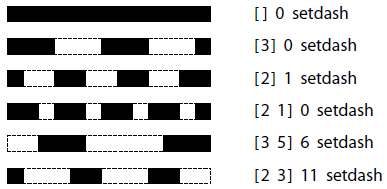
\includegraphics[width=180pt]{dash.png}}
\caption{Примеры параметров пунктирности линии}\label{pic_dash}
\end{figure}

 
Непосредственно рисованием занимаются операторы прорисовки \texttt{stroke} и операторы заливки цветом \texttt{fill} по правилу ненулевого количества поворотов (Nonzero winding number rule) и \texttt{eofill} по правилу четный-нечетный (Even-odd rule)\cite{plrm}. Операторы рисования неявно используют такие параметры, как ширину линии и цвет. Самым важным неявным параметром является \textit{текущий путь}, который изменяется при исполнении рисующего оператора. 

Для сохранения и восстановления графического состояния предусмотрены операторы \texttt{gsave} и \texttt{grestore}, которые соответственно кладут на графический стек копию графического состояния и восстанавливают сохраненное значение по копии.


\subsection{Пример программы на языке PostScript}
Для примера рассмотрим простую программу, рисующую прямоугольники, на языке PostScript: 

\iffalse
\lstset{ %
language=postscript,                 % выбор языка для подсветки (здесь это С)
basicstyle=\small\sffamily, % размер и начертание шрифта для подсветки кода
numbers=left,               % где поставить нумерацию строк (слева\справа)
numberstyle=\tiny,           % размер шрифта для номеров строк
stepnumber=1,                   % размер шага между двумя номерами строк
numbersep=5pt,                % как далеко отстоят номера строк от подсвечиваемого кода
backgroundcolor=\color{white}, % цвет фона подсветки - используем \usepackage{color}
showspaces=false,            % показывать или нет пробелы специальными отступами
showstringspaces=false,      % показывать или нет пробелы в строках
showtabs=false,             % показывать или нет табуляцию в строках
frame=single,              % рисовать рамку вокруг кода
tabsize=2,                 % размер табуляции по умолчанию равен 2 пробелам
captionpos=t,              % позиция заголовка вверху [t] или внизу [b] 
breaklines=true,           % автоматически переносить строки (да\нет)
breakatwhitespace=false, % переносить строки только если есть пробел
escapeinside={\%*}{*)}   % если нужно добавить комментарии в коде
}
\fi

%\begin{figure} [h]
%\caption{Простая программа на языке PostScript}
\begin{lstlisting}[label=PostScript-example,caption=Простая программа на языке PostScript, frame = single, language = PostScript]
% transform inches to pixels
/inch {72 mul} def

% construct a rectangle
/box        
{newpath moveto
1 inch 0 rlineto
0 1 inch rlineto
-1 inch 0 rlineto
closepath} 
def

% fill a shape with color
/fillbox {setgray fill} def

% draw three rectangels
3.5 inch 4.5 inch box
0 fillbox
3.75 inch 5 inch box
.4 fillbox
4 inch 5.5 inch box
.8 fillbox
showpage
\end{lstlisting}

Данная программа закрашивает три прямоугольника разными цветами: 

\begin{figure} [h]
\center{
\includegraphics[width=360pt]{rectangles.png}}
\caption{Результат работы программы}\label{pic_Rect}
\end{figure}
%\end{figure}


\pagebreak

\section{Реализация графической среды исполнения}
%\addcontentsline{toc}{section}{Реализация графической среды исполнения}
\sloppy

При реализации графической среды исполнения были использованы стандартные библиотеки языка Java: \texttt{jawa.awt.geom}, \texttt{jawa.awt.image} и \texttt{java.swing}. C помощью класса GeneralPath из библиотеки \texttt{jawa.awt.geom} были реализованы класс пути \texttt{PSPath} и операторы построения пути. C помощью класса JFrame из библиотеки texttt{java.swing} и класса BufferedImage из \texttt{jawa.awt.image} были реализованы рисующие операторы.

\texttt{GState} характеризует графическую среду исполнения интерпретатора PostScript. В классе хранятся такие параметры, как текущий путь \texttt{currentPath}, ограничивающий путь \texttt{clippingPath}, текущая матрица преобразования системы координат \texttt{cTM} и графические настройки \texttt{graphicsSettings}.

Текущий путь и ограничивающий путь характеризуются классом \texttt{PSPath}, реализованным с помощью стандартного класса \texttt{generalPath} из библиотеки \texttt{java.awt.geom}. По объекту PSPath можно получить ограничивающий прямоугольник \texttt{getBBox()}, сделать замкнутым текущий подпуть \texttt{closePath()} и добавить в путь отрезок \texttt{addLine()}, кривую Безье \texttt{addCurve()} и дугу эллипса \texttt{addArc()}.

Текущая матрица преобразования описывается классом \texttt{TransformMatrix}. Сама матрица представлена массивом из шести чисел в виде объекта класса \texttt{PSObject}. По экземпляру \texttt{TransformMatrix} можно изменить масштаб \texttt{scale()}, сделать пераллельный перенос \texttt{translate()} и повернуть \texttt{rotate()} систему координат, а также взять обратную матрицу \texttt{getInverseMatrix()} и по заданным относительным координатам получить абсолютные координаты \texttt{transform()}.

Графические настройки представлены классом \texttt{GraphicsSettings}, содержащим такие параметры, как цвет, ширина линии, параметры соединения отрезков и параметры пунктирной линии. 

\pagebreak
\subsection{Отображение на экране}
%\addcontentsline{toc}{section}{Отображение на экране}
\sloppy

С наглядным представлением графической среды исполнения на экране связаны такие классы, как \texttt{PSImage}, \texttt{PSFrame} и \texttt{PSDrawer}.
Класс \texttt{PSImage}, реализованный с помощью стандартного класса \texttt{java.awt.image.BufferedImage}, представляет отображение графического состояния на экране. Класс \texttt{PSDrawer} непосредственно отрисовывает графическое состояние. Объект \texttt{PSDrawer} хранит экземпляр класса \texttt{PSFrame}, наследуемого от стандартного класса \texttt{javax.swing.JFrame} и отвечающего за окно, в котором изображается графическое состояние. 


\begin{figure} [h]
\center{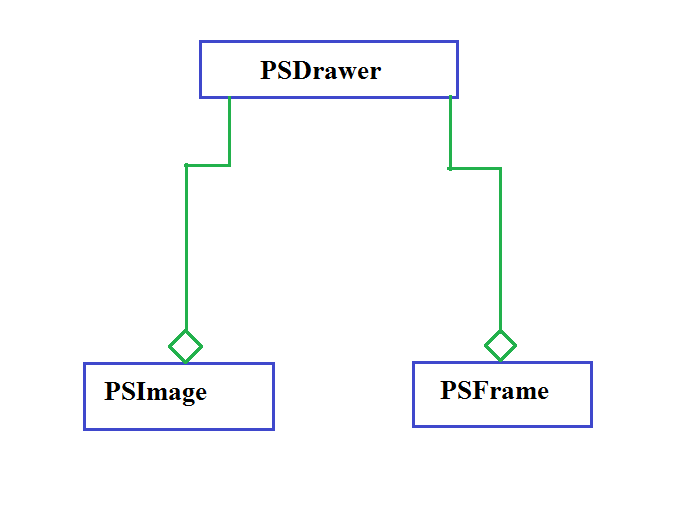
\includegraphics[width=360pt]{PSDrawer.png}}
\caption{Диаграмма классов отображения}\label{pic_Frame}
\end{figure}

\pagebreak
\subsection{Графические операторы}
%\addcontentsline{toc}{section}{Графические операторы}
\sloppy

Графические операторы, являющиеся наследниками абстрактного класса \texttt{AbstractGraphicOperator}, непосредственно воздействуют на графическое состояние.
Операторы, похожие по поведению, можно объединить в группы. Графические операторы разделяются на группы операторов графического состояния, построения пути и рисования. 

Среди операторов графического состояния есть операторы сохранения \texttt{GSaveOp()} и восстановления \texttt{GRestoreOp()} графического состояния, операторы задания цвета \texttt{SetRgbColorOp()}, ширины линии \texttt{SetLineWidth()} и параметров пунктирной линии \texttt{SetDashOp()}.

В операторы построения пути входят такие операторы, как операторы построения отрезка \texttt{LineToOp()} и \texttt{RLineToOp()}, дуги эллипса \texttt{ArcOp()} и \texttt{ArcnOp()}, кривой Безье \texttt{CurveToOp()} и \texttt{RCurveToOp()}, а также операторы перемещения текущей точки \texttt{MoveToOp()} и \texttt{RMoveToOp()}. Кроме того, можно взять ограничивающий прямоугольник пути \texttt{PathBBoxOp()}, задать новый текущий путь \texttt{NewPathOp()} и начальный ограничивающий путь \texttt{InitClipOp()}, изменить ограничивающий путь \texttt{ClipPathOp()}, а также замкнуть текущий подпуть в текущем пути \texttt{ClosePathOp()}.

Среди операторов рисования есть операторы рисования контура пути \texttt{StrokeOp()}, заливки области пути \texttt{FillOp()} и \texttt{EoFillOp()}, а также заливки области заданного прямоугольника \texttt{RectFillOp()}. 

\pagebreak

\section*{Заключение}
\addcontentsline{toc}{section}{Заключение}

В рамках курсовой работы разработана графическая среда исполнения для интерпретатора языка PostScript. В графической среде выполнения хранятся такие параметры, как текущая точка, текущий путь, ограничивающий путь,  цвет,  матрица преобразования системы координат и ширина линии. 
При этом выполнены следующие требования:
\begin{itemize}
\item Реализованы основные графические операторы.
\item Поддерживаются операторы сохранения графического состояния.
\item Есть возможность визуального представления графического состояния на 
    экране.
\item Графическая среда исполнения интерпретатора PostScript реализована на языке Java.
\end{itemize}

\bibliographystyle{ugost2008ls}
%\bibliography{expression}

\begin{thebibliography}{}
\bibitem{plrm}
PoscScript Language Reference. Third edition, 1999
\\
\url{http://www.adobe.com/products/postscript/pdfs/PLRM.pdf}

\bibitem{graphics}
Д. Роджерс, Дж. Адамс. Математические основы машинной графики. 2001. 

\end{thebibliography}


\end{document}
